\begin{document}

%----------------------------------------------------------------------------------------
%	TITLE PAGE
%----------------------------------------------------------------------------------------

\title[]{Talk 9: Operator Splitting and Federated Learning}
\date{2021-10-28}
\author[]{WEN Hao}

% \institute[北京航空航天大学] % Your institution as it will appear on the bottom of every slide, may be shorthand to save space
% {
% 数学科学学院 \\ % Your institution for the title page
% \medskip
% \textit{wenh06@gmail.com} % Your email address
% 北京航空航天大学 \\
% 数学科学学院 \qquad 北京航空航天大学
% }

% \logo{\includegraphics[height=1.5cm]{logo}}
% \logoii{\includegraphics[height=1cm]{logo2}}

% \date{\footnotesize 2021年4月13日} % Date, can be changed to a custom date

\setlength{\belowdisplayskip}{5pt} \setlength{\belowdisplayshortskip}{5pt}
\setlength{\abovedisplayskip}{5pt} \setlength{\abovedisplayshortskip}{5pt}

%------------------------------------------------

\begin{frame}
\titlepage % Print the title page as the first slide
\end{frame}

%------------------------------------------------

\section{FedSplit}

%------------------------------------------------
% Page 1

\begin{frame}
\frametitle{Motivation}

\begin{block}{The Optimization Problem}
Let $f_j$ be finite convex, with Lipschitz gradient.
\vspace{-1em}
\begin{align*}
    \text{min} & \quad F(x) := \sum_{j=1}^m f_j(x_j) \\
    \text{s.t.} & \quad x_1 = \cdots = x_m \in \mathbb{R}^d, \quad x = (x_1, \cdots, x_m)
\end{align*}
\end{block}

Main issues of existing FL algorithms (FedSGD, FedProx, etc)

\begin{itemize}
    \item Convergence
    \item {\bf Correctness}: fail to preserve the fixed points of the original optimization problem i.e. fixed points produced by the algorithm need not be stationary.
\end{itemize}

\blfootnote{
\tiny\cite{pathak2020fedsplit} \bibentry{pathak2020fedsplit}
}

\end{frame}

%------------------------------------------------
% Page 1

\begin{frame}
\frametitle{More on the Issue of Correctness (FedGD)}

\begin{prop}
The sequence $\{x^{(t)}\}^{t=1}_{\infty}$ generated by $\texttt{FedGD}(s,e)$ satisfy
\begin{itemize}
    \item if $x^{(t)}$ convergent, then $x_j^{(t)}$ share a common limit $x^*$
    \vspace{-0.3em}
    \item $x^*$ satisfy the fixed point relation {\smaller$\sum\limits_{i=1}^e\sum\limits_{j=1}^m \nabla f_j(G_j^{i-1}(x^*)) = 0$}
\end{itemize}
\end{prop}

\begin{block}{Notations (\texttt{FedGD})}
\begin{itemize}
\item $G_j(x_j) := x_j - s\nabla f_j(x_j)$ the gradient mappings
\item $G^e_j(x_j) := \underbrace{G_j\circ\cdots\circ G_j}_{e-\text{times}} (x_j)$
\item $x_j^{(t+1/2)} := G^e_j(x_j^{(t)})$, $x_j^{(t+1)} = \overline{x}^{(t+1/2)}:=\frac{1}{m}\sum\limits_{j=1}^m x_j^{(t+1/2)}.$
\end{itemize}
\end{block}

\end{frame}

%------------------------------------------------
% Page 1

\begin{frame}
\frametitle{More on the Issue of Correctness (FedGD)}

Note the abuse of the notation $x$!

Sketch:

Assume $x^{(t)} = (x_1^{(t)}, \cdots, x_m^{(t)}) \to (x_1^{*}, \cdots, x_m^{*})$, then
$$(x_1^{*}, \cdots) = \texttt{FedGD}(s,e)(x_1^{*}, \cdots) = \left(\frac{1}{m}\sum\limits_{j=1}^m G^e_j(x_j^{*}), \cdots \right)$$
% \vspace{-1em}
Hence $x_1^{*} = \cdots = x_m^{*} = x^{*}.$ Write $\frac{1}{m}\sum_{j=1}^m G^e_j(x^{*}) = x^{*}$, and substitute $G^e_j$ by its definition, one has
\vspace{-0.7em}
$$\sum\limits_{i=1}^e\sum\limits_{j=1}^m \nabla f_j(G_j^{i-1}(x^*)) = 0.$$

\end{frame}

%------------------------------------------------
% Page 1

\begin{frame}
\frametitle{More on the Issue of Correctness (FedGD)}

Indeed, one has
{\smaller
\begin{align*}
0 = & \frac{1}{m}\sum_{j=1}^m G^e_j(x^{*}) - x^{*} \\
= & \frac{1}{m}\sum_{j=1}^m \left( G^{e-1}_j(x^{*}) - s\nabla F_j (G^{e-1}_j(x^{*})) \right) - x^{*} \\
= & \frac{1}{m}\sum_{j=1}^m G^{e-1}_j(x^{*}) - x^{*} - \frac{s}{m}\sum_{j=1}^m\nabla F_j (G^{e-1}_j(x^{*})) \\
& \hspace{3em} \vdots \\
= & \frac{1}{m}\sum_{j=1}^m G^{0}_j(x^{*}) - x^{*} - \frac{s}{m}\sum\limits_{i=1}^e\sum\limits_{j=1}^m \nabla f_j(G_j^{i-1}(x^*)) \\
= & - \frac{s}{m}\sum\limits_{i=1}^e\sum\limits_{j=1}^m \nabla f_j(G_j^{i-1}(x^*))
\end{align*}
}

\end{frame}

%------------------------------------------------
% Page 1

\begin{frame}
\frametitle{More on the Issue of Correctness (FedProx)}

\begin{prop}
The sequence $\{x^{(t)}\}^{t=1}_{\infty}$ generated by $\texttt{FedProx}$ satisfy
\begin{itemize}
    \item if $x^{(t)}$ convergent, then $x_j^{(t)}$ share a common limit $x^*$
    \vspace{-0.3em}
    \item $x^*$ satisfy the fixed point relation {$\sum\limits_{j=1}^m \nabla M_{sf_j}(x^*) = 0$}
\end{itemize}
\end{prop}

\begin{block}{Notations (\texttt{FedProx})}
\begin{itemize}
\item $\operatorname{prox}_{sf_j} (z) := \argmin\limits_{x_j} \left\{ f_j(x_j) + \frac{1}{2s} \lVert z-x_j \rVert^2 \right\}$
\vspace{-0.3em}
\item $M_{sf_j} := \inf\limits_x \left\{ f_j(x_j) + \frac{1}{2s} \lVert z-x_j \rVert^2 \right\}$
\vspace{-0.3em}
\item $x_j^{(t+1/2)} := \operatorname{prox}_{sf_j}(x_j^{(t)})$, $x_j^{(t+1)} = \overline{x}^{(t+1/2)}.$
\end{itemize}
\end{block}

\end{frame}

%------------------------------------------------
% Page 1

\begin{frame}
\frametitle{More on the Issue of Correctness (FedProx)}

Sketch:

As $f_j$ are smooth convex, one has
$$\operatorname{prox}_{sf_j}(z) = z - s\nabla M_{sf_j}(z)$$
Hence
{\smaller
\begin{align*}
0 & = x^* - \frac{1}{m}\sum_{j=1}^m \operatorname{prox}_{sf_j}(x^*) \\
& = x^* - \frac{1}{m}\sum_{j=1}^m \left( x^* - s\nabla M_{sf_j}(x^*) \right) \\
& = x^* - \frac{1}{m}\sum_{j=1}^m x^* + \frac{s}{m}\sum_{j=1}^m\nabla M_{sf_j}(x^*) \\
& = \frac{s}{m}\sum_{j=1}^m\nabla M_{sf_j}(x^*)
\end{align*}
}

\end{frame}

%------------------------------------------------
% Page 1

\begin{frame}
\frametitle{Incorrectness for Least Square Problems}

\begin{block}{Least Square Problem (LSP)}
$f_j(x_j) = \frac12 \lVert A_jx_j-b_j \rVert^2$, and $A_j$ has full rank ($=d$).
\end{block}

LSP has unique solution
{\smaller
$$x^*_{ls} = \left( \sum_{j=1}^m A_j^TA_j \right)^{-1} \sum_{j=1}^m A_j^Tb_j$$
}

\pause

By previous propositions,
\begin{itemize}
    \item {\smaller$x^*_{\texttt{FedGD}} = \left( \sum\limits_{j=1}^m A_j^TA_j G \right)^{-1}\left( \sum\limits_{j=1}^m GA_j^Tb_j \right)$, with $G = \sum\limits_{k=0}^{e-1}(I-sA_j^TA_j)^k$}
    \item {\smaller$x^*_{\texttt{FedProx}} = \left( \sum\limits_{j=1}^m \left( I - P_j \right) \right)^{-1}\left( \frac{1}{s}\sum\limits_{j=1}^m P_jA_j^Tb_j \right)$, with $P_j = (I+sA_j^TA_j)^{-1}$}
\end{itemize}

\end{frame}

%------------------------------------------------
% Page 1

\begin{frame}
\frametitle{Incorrectness for Least Square Problems}

Settings: $m=25$, $d=100$, $A_j \in \operatorname{Mat}_{500\times 100}$, $(A_j)_{kl} \sim N(0,1)$, $b_j = A_jx_0 + \varepsilon_j$ with $\varepsilon_j \sim N(0,0.25I)$

\begin{figure}
\centering
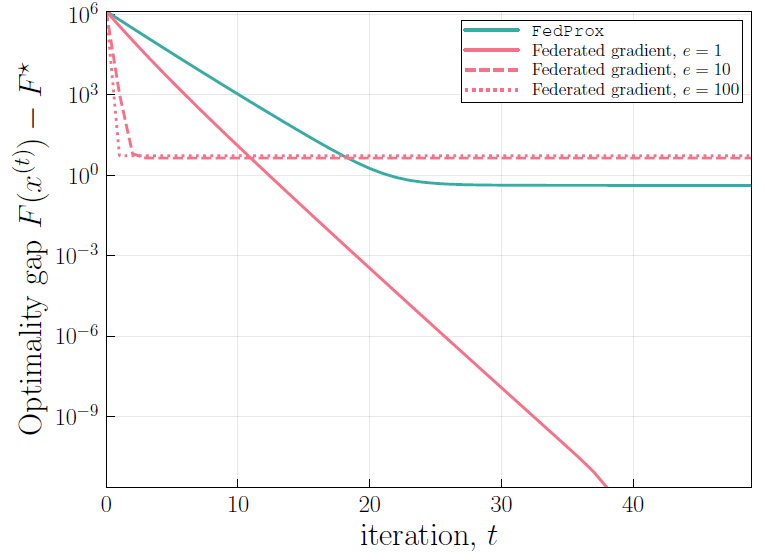
\includegraphics[width=0.8\textwidth]{images/fedsplit-gap.png}
\end{figure}

\end{frame}

%------------------------------------------------
% Page 1

\begin{frame}
\frametitle{FedSplit - Problem Reformulation}

The original problem can be reformulated as
\begin{align*}
    \text{min} & \quad F(x) := \sum_{j=1}^m f_j(x_j) \\
    \text{s.t.} & \quad Ax = 0
\end{align*}
where $x = (x_1, \cdots, x_m), A = \text{{\smaller[3]$\begin{pmatrix} I & -I & & & & \\ & I & -I & & \\ & & \ddots & \ddots & \\ & & & \ddots & -I \\ -I & & & & I \end{pmatrix}$}}$

Consider the first-order optimal condition for $L(x,y) = F(x) - \langle y, Ax \rangle$, i.e. $\nabla F(x) - A^Ty = 0$, or equiv.
$$\nabla F(x) - \begin{pmatrix} y_1-y_m \\ \vdots \\ y_m-y_{m-1} \end{pmatrix} = 0$$

\end{frame}

%------------------------------------------------
% Page 1

\begin{frame}
\frametitle{FedSplit - Problem Reformulation}

Hence is a monotone inclusion problem
$$0 \in \nabla F(x) + \mathcal{N}_E(x)$$
where
\begin{align*}
\mathcal{N}_E(x) & = \begin{cases} E^{\perp} & \text{ if } x \in E \\ \emptyset & \text{ otherwise } \end{cases} \text{normal cone} \\
E & = \{x \ |\ x_1 = \cdots = x_m\}
\end{align*}
Indeed for $x\in E$,
\begin{align*}
\mathcal{N}_E(x) & = \left\{ y \ \middle|\ \langle y, \widetilde{x} - x \rangle \leqslant 0 \ \forall \widetilde{x} \in E \right\} \\
& = \left\{ y \ \middle|\ \langle \sum\nolimits_{j=1}^m y_j, \widetilde{x}_1 - x_1 \rangle \leqslant 0 \ \forall \widetilde{x}_1 \in \mathbb{R}^d \right\} \\
& = \left\{ y \ \middle|\ \sum\nolimits_{j=1}^m y_j = 0 \right\} = E^{\perp}
\end{align*}

\end{frame}

%------------------------------------------------
% Page 1

\begin{frame}
\frametitle{FedSplit - Problem Reformulation}

\begin{block}{Another Perspective of Problem Reformulation}
Let $\iota_E$ be the indicator function of $E$, then the constrained problem can be reformulated as the following unconstrained one
$$\min \ F(x) + \iota_E(x), \quad x \in \mathbb{R}^{md}$$
The first-order optimal condition gives
$$0 \in \nabla F(x) + \partial \iota_E(x) = \nabla F(x) + \mathcal{N}_E(x)$$
\end{block}

\end{frame}

%------------------------------------------------
% Page 1

\begin{frame}
\frametitle{FedSplit - Operator Splitting}

Let $\mathcal{F} = A+B$, with $A$, $B$ maximal monotone. Write
\begin{gather*}
R_A = (I + s A)^{-1}, \quad R_B = (I + s B)^{-1} \\
C_A = 2R_A - I, \quad C_B = 2R_B - I
\end{gather*}
Then
\begin{itemize}
    \item $C_A, C_B, C_AC_B$ nonexpansive
    \item $0\in A(x)+B(x) \Longleftrightarrow C_AC_B(z) = z, \ x = R_B(z)$
\end{itemize}
i.e. we are reduced to finding fixed points of the nonexpansive operator $ C_AC_B$.

\end{frame}

%------------------------------------------------
% Page 1

\begin{frame}
\frametitle{FedSplit - Operator Splitting}

Now consider $\mathcal{F} = \nabla F + \mathcal{N}_E$, one is reduced to find fixed points of $C_AC_B$ with $A = \nabla F$, $B = \mathcal{N}_E$. One has
$$R_{\nabla F} = \operatorname{prox}_{sF}, \quad R_{\mathcal{N}_E} = \Pi_{E}$$
and
\begin{align*}
\operatorname{prox}_{sF}(x) & = \argmin_z \left\{ F(z) + \frac{1}{2s} \lVert z-x \rVert^2 \right\} \\
& = \argmin_z \left\{ \sum_{j=1}^m f_j(z_j) + \frac{1}{2s} \sum_{j=1}^m \lVert z_j-x_j \rVert^2 \right\} \\
& = (\operatorname{prox}_{sf_j}(x_j))_{j=1}^m
\end{align*}

\end{frame}

%------------------------------------------------
% Page 1

\begin{frame}
\frametitle{FedSplit - Operator Splitting}

\begin{itemize}
    \item Peaceman-Rachford splitting
    $$z^{(t+1)} = C_A C_B(z^{(t)})$$
    \item Douglas-Rachford splitting
    $$z^{(t+1)} = \frac12(I + C_A C_B)(z^{(t)})$$
\end{itemize}

\vspace{-0.8em}

\begin{columns}
\begin{column}{0.4\textwidth}
\begin{block}{Peaceman-Rachford}
\ 
\vspace{-1.3em}
\begin{align*}
x^{(t+1/2)} & = R_B(z^{(t)}) \\
z^{(t+1/2)} & = 2x^{(t+1/2)} - z^{(t)} \\
x^{(t+1)} & = R_A(z^{(t+1/2)}) \\
z^{(t+1)} & = z^{(t)} + 2x^{(t+1)} \\
& \phantom{=} - 2x^{(t+1/2)}
\end{align*}
\end{block}
\end{column}
\begin{column}{0.4\textwidth}
\begin{block}{Douglas-Rachford}
\ 
\vspace{-1.3em}
\begin{align*}
x^{(t+1/2)} & = R_B(z^{(t)}) \\
z^{(t+1/2)} & = 2x^{(t+1/2)} - z^{(t)} \\
x^{(t+1)} & = R_A(z^{(t+1/2)}) \\
z^{(t+1)} & = z^{(t)} + x^{(t+1)} \\
& \phantom{=} - x^{(t+1/2)}
\end{align*}
\end{block}
\end{column}
\end{columns}

\end{frame}

%------------------------------------------------
% Page 1

\begin{frame}
\frametitle{FedSplit - The Algorithm}

{
\smaller
\begin{algorithm}[H]
\SetAlgoNoLine
\DontPrintSemicolon
{\bfseries Given} initiation $x\in\mathbb{R}^d$, proximal solvers $\texttt{prox\_update}_j: \mathbb{R}^d \to \mathbb{R}^d$ \;
{\bfseries Initialize} $x^{(1)} = z_1^{(1)} = \cdots = z_m^{(1)} = x$\;
\For{$t = 1, 2, \cdots$}{
    \For{$j = 1, \cdots, m$ {\bfseries in parallel}}{
        Local prox step: $z_j^{(t+1/2)} \gets$ $\texttt{prox\_update}_j(2x^{(t)} - z_j^{(t)})$\;
        Local centering step: $z_j^{(t+1)} \gets$ $z_j^{(t)} + 2(z_j^{(t+1/2)} - x^{(t)})$
        }
    Compute global average: $x^{(t+1)} \gets \overline{z}^{(t+1)}$\;
    \If{meet convergent criteria}{
        $x^* \gets x^{(t+1)}$\;
        {\bfseries break}\;
    }
}
return $x^*$\;
\caption{FedSplit}
\end{algorithm}
}

Note the difference against previous iteration form of Peaceman-Rachford:
\begin{center}
first step -> last step; 2, 3 step merges; parameters renamed
\end{center}

\end{frame}

%------------------------------------------------
% Page 1

\begin{frame}
\frametitle{FedSplit - Correctness and Convergence}

\begin{prop}[Correctness]
If $z^* = (z_1^*, \cdots, z_m^*)$ is a fixed point of \texttt{FedSplit}, then $x^* := \Pi_E(z^*) = \frac{1}{m} \sum_{j=1}^m z_j^*$ is an optimal solution to the original problem $\min\limits_{x} \sum_{j=1}^m f_j(x)$.
\end{prop}

\begin{thm}[Convergence]
Let $f_j$ be $\ell_j$-strongly convex and $L_j$-smooth, $\ell_* = \min \ell_j$, $L^* = \max L_j$, $\kappa = L^*/\ell_*$. {\color{red} Take step size $s = 1 / \sqrt{\ell_*L^*}$}, and assume $\lVert \texttt{prox\_update}_j(z) - \operatorname{prox}_{sf_j}(z) \rVert \leqslant b$, then
$$\lVert x^{(t+1)} - x^* \rVert \leqslant \left( 1 - \frac{2}{\sqrt{\kappa}+1} \right)^t \frac{\lVert z^{(1)} - z^* \rVert}{\sqrt{m}} + (\sqrt{\kappa}+1)b$$
\end{thm}

\end{frame}

%------------------------------------------------
% Page 1

\begin{frame}
\frametitle{FedSplit - Non Strongly Convex Case}

Consider a suitable regularization
\begin{align*}
\min & F_{\lambda}(z) = \sum_{j=1}^m \left( f_j(z_j) + \frac{\lambda}{2}\lVert z_j - x^{(1)} \rVert^2 \right) \\
\text{s.t.} & z_1 = \cdots z_m
\end{align*}

\begin{thm}
Let $\lambda \in \left(0, \frac{\varepsilon}{m\lVert x^* - x^{(1)} \rVert^2}\right)$, error bound $F(\widehat{x}) - F^* \leqslant \varepsilon$, \texttt{FedSplit} with regularized objective $F_{\lambda}$ and step size $s = 1/\sqrt{\lambda(L^*+\lambda)}$ converges in at most
$$O \left( \sqrt{\frac{L^*\lVert x^* - x^{(1)} \rVert^2}{\varepsilon}} \right)$$
iterations
\end{thm}

\end{frame}

%------------------------------------------------

\section{FedDR}

%------------------------------------------------
% Page 1

\begin{frame}
\frametitle{Motivation and Formulation}

\begin{block}{Motivation}
\begin{itemize}
    \item Nonconvex Douglas-Rachford splitting
    \item randomized block-coordinate strategy
\end{itemize}
\end{block}

\begin{block}{Problem Formulation}
\ 
\vspace{-1.3em}
$$\min_x F(x) = f(x) + g(x) = \frac{1}{n} \sum_{i=1}^n f_i(x) + g(x)$$
\vspace{-1.3em}
\begin{itemize}
    \item $f_i$ nonconvex, $L$-smooth,
    \item $g$ closed proper convex
\end{itemize}
\end{block}


\blfootnote{
\tiny\cite{tran2021feddr} \bibentry{tran2021feddr}
}

\end{frame}

%------------------------------------------------
% Page 1

\begin{frame}[allowframebreaks]
\frametitle{References}

{\footnotesize
\bibliographystyle{ieeetr}
\bibliography{references}
}

\end{frame}

%------------------------------------------------

\end{document}
